Saddle-Node-Bifurkation &
$\dot x = r + x^2 \quad r\in\mathbb{R} \qquad f(x^*) = r+(x^*)^2 + r = 0 \implies x^*_{1,2} = \pm \sqrt{-r}$\newline 
$f'(x^*) = 2x^* = \begin{cases}> 0 & 2\cdot\sqrt{-r} \quad \text{instabile Fixpunkte}\\<0 &-2\cdot\sqrt{-r} \quad \text{stabile Fixpunkte}\end{cases}$
\\
&
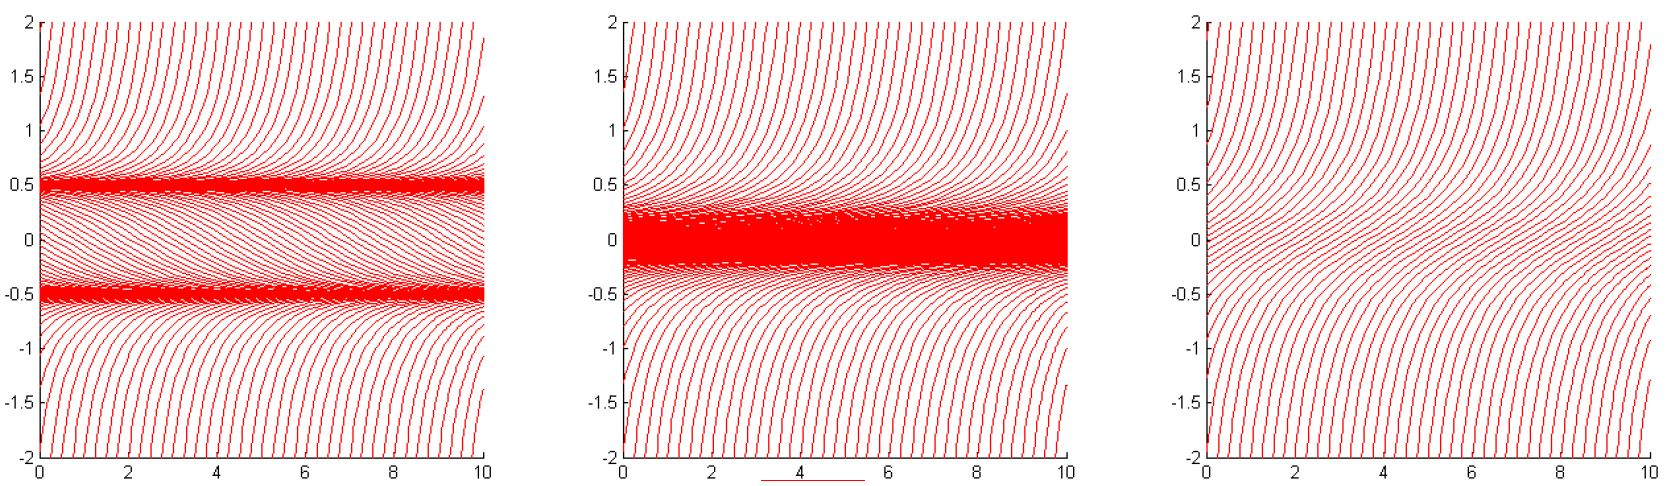
\includegraphics[scale = .15]{images/bif_saddle_node} 
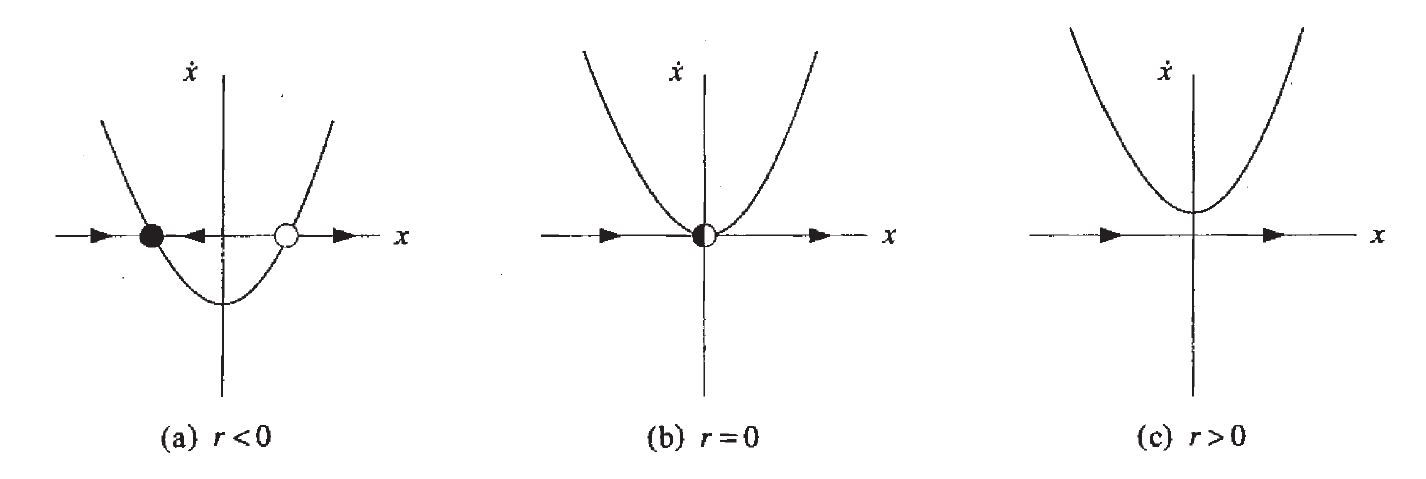
\includegraphics[scale = .15]{images/bif_saddle_node2} 
\\